\section{Ingestion module for the MPL\_NPPF file}

This sections describes the ingestion module for inserting the planning of operations commanding the satellite.

The associated ingestion processor is:

\begin{itemize} 

\item \textbf{s2boa.ingestions.ingestion\_nppf.ingestion\_nppf}
  
\end{itemize}

This module uses the following \acrshort{dim} signatures:

\begin{itemize} 

\item \textbf{NPPF\_XXX}: data corresponding to the planning of operations commanding the satellite.

\item \textbf{CORRECTED\_NPPF\_XXX}: data corresponding to the planning of operations commanding the satellite corrected by the available orbit prediction data.

\item \textbf{COMPLETENESS\_NPPF\_XXX}: data corresponding to the definition of planning completeness used for analysis.
  
\end{itemize}

Where XXX is the corresponding satellite id.

The figure \ref{fg:structure_ingestion_nppf} shows a simplified diagram of the structure of events inserted (associated structure of values not included for simplicity).

\begin{figure}[H]
  \begin{center}
	\centering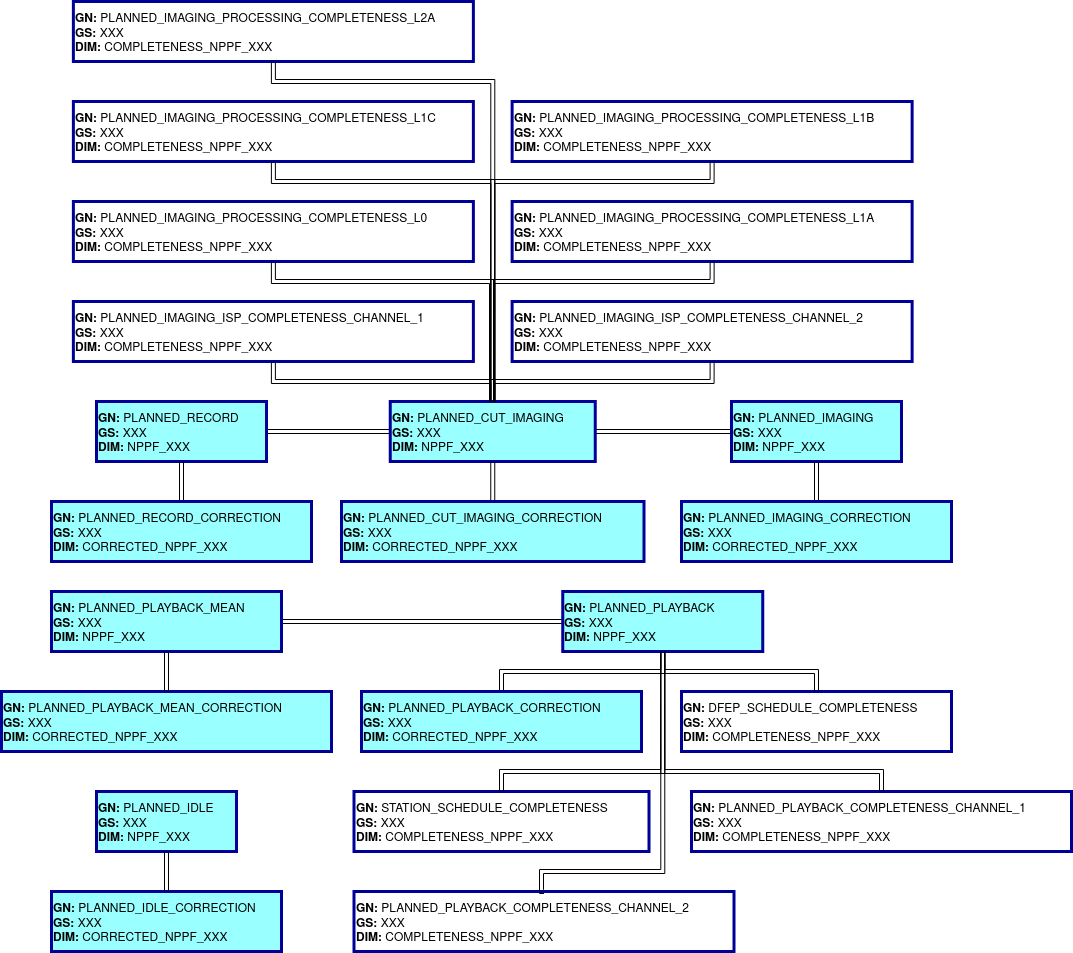
\includegraphics[width=150mm]{../fig/structure_ingestion_nppf.png}
	\caption{Structure of events inserted by the ingestion module for the MPL\_NPPF file}
	\label{fg:structure_ingestion_nppf}
  \end{center}
\end{figure}

The table \ref{tb:description_events_ingestion_nppf} shows the description of the events inserted by the ingestion.

\begin{landscape}
\begin{longtable}{|M{0.15\linewidth}|M{0.05\linewidth}|M{0.10\linewidth}|M{0.10\linewidth}|M{0.15\linewidth}|M{0.15\linewidth}|M{0.15\linewidth}|}
\hline \textbf{Gauge name} & \textbf{Gauge system} & \textbf{DIM signature} & \textbf{Insertion mode} & \textbf{Description} & \textbf{Start} & \textbf{Stop} \\ \hline
\textbf{PLANNED\_RECORD} & XXX & NPPF\_XXX & ERASE\_and\_REPLACE (insert\_and\_erase) & Event for representing the \textbf{recording operation} & UTC time associated to command 'MPMMRNOM' or 'MPMMRNRT' & UTC time associated to command 'MPMMRSTP' or 'MPMMRNRT' or 'MPMMRNOM' \\ \hline
\textbf{PLANNED\_CUT\_IMAGING} & XXX & NPPF\_XXX & ERASE\_and\_REPLACE (insert\_and\_erase) & Event for representing the \textbf{imaging operation associated to a specific recording operation} & UTC time associated to command 'MPMSSCAL' or 'MPMSDASC' or 'MPMSDCLO' or 'MPMSIVIC' or 'MPMSNOBS' or 'MPMSIRAW' or 'MPMSIDTS' or 'MPMMRNOM' or 'MPMMRNRT' & UTC time associated to command 'MPMSIMID' or 'MPMSIDSB' or 'MPMMRSTP' or 'MPMMRNRT' or 'MPMMRNOM' \\ \hline
\textbf{PLANNED\_IMAGING} & XXX & NPPF\_XXX & ERASE\_and\_REPLACE (insert\_and\_erase) & Event for representing the \textbf{imaging operation} covering one or several planned recording operations & UTC time associated to command 'MPMSSCAL' or 'MPMSDASC' or 'MPMSDCLO' or 'MPMSIVIC' or 'MPMSNOBS' or 'MPMSIRAW' or 'MPMSIDTS' & UTC time associated to command 'MPMSIMID' or 'MPMSIDSB' or 'MPMMRSTP' \\ \hline
\textbf{PLANNED\_PLAYBACK} & XXX & NPPF\_XXX & ERASE\_and\_REPLACE (insert\_and\_erase) & Event for representing the \textbf{playback operation} & UTC time associated to command 'MPMMPNOM' or 'MPMMPREG' or 'MPMMPBRT' or 'MPMMPNRT' & UTC time associated to command 'MPMMPSTP' \\ \hline
\textbf{PLANNED\_PLAYBACK\_MEAN} & XXX & NPPF\_XXX & ERASE\_and\_REPLACE (insert\_and\_erase) & Event for representing the \textbf{mean of the playback operation} & UTC time associated to command 'MPXBSBOP' or 'MPG1STRT' or 'MPG2STRT' & UTC time associated to command 'MPXBOPSB' (when start is associated to command 'MPXBSBOP') or 'MPOCPRY2' (when start is associated to command 'MPG1STRT' or 'MPG2STRT') \\ \hline
\textbf{PLANNED\_IDLE} & XXX & NPPF\_XXX & ERASE\_and\_REPLACE (insert\_and\_erase) & Event for representing the \textbf{idle state} & UTC time associated to command 'MPMSIMID' or 'MPMSSBID' & UTC time associated to command 'MPMSSCAL' or 'MPMSDASC' or 'MPMSDCLO' or 'MPMSIVIC' or 'MPMSNOBS' or 'MPMSIRAW' or 'MPMSIDTS' or 'MPMSIDSB' \\ \hline
\textbf{***\_CORRECTION} & XXX & \- CORRECTED\_NPPF\_XXX & ERASE\_and\_REPLACE (insert\_and\_erase) & Event for representing the \textbf{planning events corrected using the orbit prediction events} & Start of the planned event corrected using the ORBPRE & Stop of the planned event corrected using the ORBPRE \\ \hline
\textbf{DFEP\_SCHEDULE\_COMPLETENESS} & XXX & \- COMPLETENESS & ERASE\_and\_REPLACE (insert) & Event for representing the \textbf{expectation of the DFEP schedule} & Corrected start of the planned playback + 2s (SAD/HKTM) or + 9s (MSI); (if start \textgreater  stop) Corrected stop of the planned playback - 4s & Start (SAD/HKTM) or Corrected stop of the planned playback - 9s (MSI); (if start \textgreater  stop) Corrected stop of the planned playback - 3s \\ \hline
\textbf{STATION\_SCHEDULE\_COMPLETENESS} & XXX & \- COMPLETENESS\_NPPF\_XXX & ERASE\_and\_REPLACE (insert) & Event for representing the \textbf{expectation of the Station schedule} & Corrected start of the planned playback + 2s (SAD/HKTM) or + 9s (MSI); (if start \textgreater  stop) Corrected stop of the planned playback - 4s & Start (SAD/HKTM) or Corrected stop of the planned playback - 9s (MSI); (if start \textgreater  stop) Corrected stop of the planned playback - 3s \\ \hline
\textbf{PLANNED\_PLAYBACK\_COMPLETENESS\_CHANNEL\_1} & XXX & \- COMPLETENESS\_NPPF\_XXX & ERASE\_and\_REPLACE (insert) & Event for representing the \textbf{expectation of the planned playbacks using the channel 1} & Corrected start of the planned playback + 2s (SAD/HKTM) or + 9s (MSI); (if start \textgreater  stop) Corrected stop of the planned playback - 4s & Start (SAD/HKTM) or Corrected stop of the planned playback - 9s (MSI); (if start \textgreater  stop) Corrected stop of the planned playback - 3s \\ \hline
\textbf{PLANNED\_PLAYBACK\_COMPLETENESS\_CHANNEL\_2} & XXX & \- COMPLETENESS\_NPPF\_XXX & ERASE\_and\_REPLACE (insert) & Event for representing the \textbf{expectation of the planned playbacks using the channel 2} & Corrected start of the planned playback + 2s (SAD/HKTM) or + 9s (MSI); (if start \textgreater  stop) Corrected stop of the planned playback - 4s & Start (SAD/HKTM) or Corrected stop of the planned playback - 9s (MSI); (if start \textgreater  stop) Corrected stop of the planned playback - 3s \\ \hline
\textbf{PLANNED\_IMAGING\_ISP\_COMPLETENESS\_CHANNEL\_1} & XXX & \- COMPLETENESS\_NPPF\_XXX & ERASE\_and\_REPLACE (insert) & Event for representing the \textbf{expectation of the planned imaging using the channel 1} & Corrected start of the planned imaging + 10s; (if start \textgreater  stop) Corrected stop of the planned imaging - 12s & Corrected stop of the planned imaging - 10s; (if start \textgreater  stop) Corrected stop of the planned imaging - 6s \\ \hline
\textbf{PLANNED\_IMAGING\_ISP\_COMPLETENESS\_CHANNEL\_2} & XXX & \- COMPLETENESS\_NPPF\_XXX & ERASE\_and\_REPLACE (insert) & Event for representing the \textbf{expectation of the planned imaging using the channel 2} & Corrected start of the planned imaging + 10s; (if start \textgreater  stop) Corrected stop of the planned imaging - 12s & Corrected stop of the planned imaging - 10s; (if start \textgreater  stop) Corrected stop of the planned imaging - 6s \\ \hline
\textbf{PLANNED\_IMAGING\_PROCESSING\_COMPLETENESS\_L0} & XXX & \- COMPLETENESS\_NPPF\_XXX & ERASE\_and\_REPLACE (insert) & Event for representing the \textbf{expectation of the processing of the planned imaging for the L0} & Corrected start of the planned imaging + 10s; (if start \textgreater  stop) Corrected stop of the planned imaging - 12s & Corrected stop of the planned imaging - 10s; (if start \textgreater  stop) Corrected stop of the planned imaging - 6s \\ \hline
\textbf{PLANNED\_IMAGING\_PROCESSING\_COMPLETENESS\_L1A} & XXX & \- COMPLETENESS\_NPPF\_XXX & ERASE\_and\_REPLACE (insert) & Event for representing the \textbf{expectation of the processing of the planned imaging for the L1A} & Corrected start of the planned imaging + 10s; (if start \textgreater  stop) Corrected stop of the planned imaging - 12s & Corrected stop of the planned imaging - 10s; (if start \textgreater  stop) Corrected stop of the planned imaging - 6s \\ \hline
\textbf{PLANNED\_IMAGING\_PROCESSING\_COMPLETENESS\_L1B} & XXX & \- COMPLETENESS\_NPPF\_XXX & ERASE\_and\_REPLACE (insert) & Event for representing the \textbf{expectation of the processing of the planned imaging for the L1B} & Corrected start of the planned imaging + 10s; (if start \textgreater  stop) Corrected stop of the planned imaging - 12s & Corrected stop of the planned imaging - 10s; (if start \textgreater  stop) Corrected stop of the planned imaging - 6s \\ \hline
\textbf{PLANNED\_IMAGING\_PROCESSING\_COMPLETENESS\_L1C} & XXX & \- COMPLETENESS\_NPPF\_XXX & ERASE\_and\_REPLACE (insert) & Event for representing the \textbf{expectation of the processing of the planned imaging for the L1C} & Corrected start of the planned imaging + 10s; (if start \textgreater  stop) Corrected stop of the planned imaging - 12s & Corrected stop of the planned imaging - 10s; (if start \textgreater  stop) Corrected stop of the planned imaging - 6s \\ \hline
\textbf{PLANNED\_IMAGING\_PROCESSING\_COMPLETENESS\_L2A} & XXX & \- COMPLETENESS\_NPPF\_XXX & ERASE\_and\_REPLACE (insert) & Event for representing the \textbf{expectation of the processing of the planned imaging for the L2A} & Corrected start of the planned imaging + 10s; (if start \textgreater  stop) Corrected stop of the planned imaging - 12s & Corrected stop of the planned imaging - 10s; (if start \textgreater  stop) Corrected stop of the planned imaging - 6s \\ \hline
\caption{Table describing the events associated to the ingestion}
\label{tb:description_events_ingestion_nppf}
\end{longtable}
\end{landscape}

\subsection{Ingestion details}

This section describes some ingestion details for inserting the data. In particular:

\begin{itemize} 

\item The correction of the generation time when is greater than the validity start
  
\end{itemize}

\subsubsection{Correction of the generation time}

Due to an operation procedure using the \acrshort{s2mp}, the generation time could be greater than the validity start. This could result into having deprecated data in the DDBB.

To solve this issue the processor changes the generation time to be the validity start when the first is greater.
